\chapter*{Week 15: Sorting Algorithms and Recursion}
\addcontentsline{toc}{chapter}{Week 15: Sorting Algorithms and Recursion}
\setcounter{chapter}{15}
\setcounter{section}{0}

%Skip week 14 -- Thanksgiving

\begin{abstract}
This week you will:
\begin{enumerate}
    \item Learn about pass by reference parameters
    \item Learn about sorting algorithms and how to discuss the ``speed" of an algorithm
    \item Learn how to use recursive functions

\end{enumerate}
    
\end{abstract}

\section{Background}

\subsection{Pass By Reference Parameters}

In C++, you can pass parameters to functions either by value or by reference. Passing by reference allows you to modify the original variable within the function.

The basic syntax is:

\begin{minted}{c++}
void functionName(<data_type> &parameter_name)
{
    // Function body
}
\end{minted}

\begin{example}
    \begin{minted}{c++}

    
#include <iostream>
using namespace std;

// Function to increment a number by value
void incrementByValue(int num)
{
    num++;
}

// Function to increment a number by reference
void incrementByReference(int &num)
{
    num++;
}

int main()
{
    int x = 5;

    cout << "Before increment: " << x << endl;
    incrementByValue(x); // passing x by value
    cout << "After increment: " << x << endl;

    cout << "---" << endl;

    cout << "Before increment: " << x << endl;
    incrementByReference(x); // passing x by reference
    cout << "After increment: " << x << endl;

    return 0;
}
    \end{minted}
\end{example}

\begin{sample}
Before increment: 5 \\
After increment: 5\\
---\\
Before increment: 5\\
After increment: 6\\
\end{sample}

Key points to remember:

\begin{itemize}
    \item Parameters passed by reference are indicated by \& in the function declaration.
    \item Changes made to the reference parameter within the function affect the original variable.
    \item Pass by reference avoids unnecessary copying of the argument to the parameter variable, which can be more efficient.
    \item Arrays are passed by reference by default (so there is no preceding \& for an array parameter).
    \item References cannot be reassigned to refer to a different variable once initialized.
\end{itemize}
    
\subsection{Sorting Algorithms}

There are several different strategies to sort unordered lists of data. They generally fall into two categories based on how long it takes for them to run proportionate to the number of items they are designed to sort. 

When discussing how long an algorithm takes to run, we use something called ``Big O Notation". To use Big O, you need to determine the size of the input, which is designated as $n$. The number of singular operations to execute your algorithm as a function of the input size defines how long it takes -- for example if you have to look at every element in your list only once, you would need $n$ operations. If you had to compare every element to every other element in your list, you would need $n^2$ operations. Big O then removes any constants or smaller terms, as we are only concerned with the limit of the behavior -- i.e., what happens as your input gets exceedingly large. 

When using Big-O, the two categories of sorting algorithms become clear: algorithms that generally either require that you compare every element against every other element, meaning they take $O(n^2)$ time, or algorithms that continuously break your data set in halves and compare these smaller pieces, which would take $O(n*log(n))$ time, as seen in Quick Sort.

\subsubsection{Bubble Sort}

Bubble Sort is generally considered the simplest sorting algorithm. It works by repeatedly swapping the adjacent elements if they are in the wrong order, only comparing two at a time.

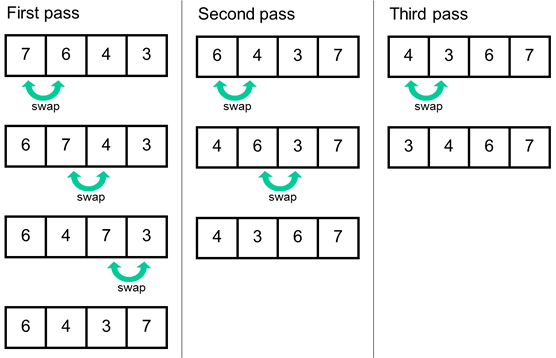
\includegraphics[width=\textwidth]{images/bubble_sort.png}
Image Source: https://www.computersciencebytes.com/sorting-algorithms/bubble-sort/

Bubble sort requires comparing $n$ elements against $n$ elements, and so its computational complexity described using Big-O is $O(n^2)$.

\subsubsection{Selection Sort}

Selection Sort involves picking the smallest (or largest) number out of the unsorted elements and then putting it in its own list, one after the other, so that you find the smallest, then the second smallest, and so on and so forth. 

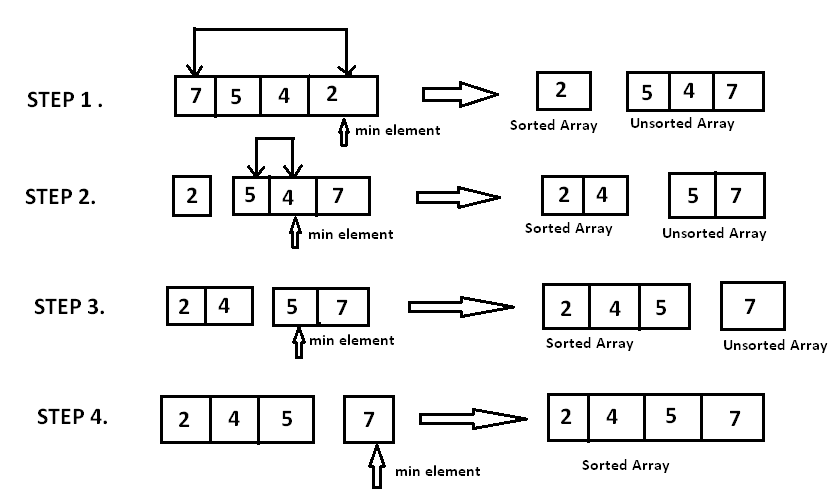
\includegraphics[width=\textwidth]{images/selection-sort.png}
Image Source: https://www.hackerearth.com/practice/algorithms/sorting/selection-sort/tutorial/

For the first level of selection sort, you must search all $n$ elements to find the smallest one. For the second level, you must search $n-1$ elements, then $n-2$, and so on and so forth. This will ultimately require $\frac{n^2}{2}$ operations. We do not worry about constants such as $\frac{1}{2}$ in Big-O, and so this is still a computational complexity of $O(n^2)$.

Below are four algorithms chosen to represent the different styles of sorting algorithms available to you.

\subsubsection{Insertion Sort}

Insertion sort works by splitting the list of elements into two pieces: one piece that has already been sorted, and one piece that has not been sorted yet. The algorithm goes through the unsorted list one element at a time and inserts it into the correct position in the sorted list until all elements have been sorted.

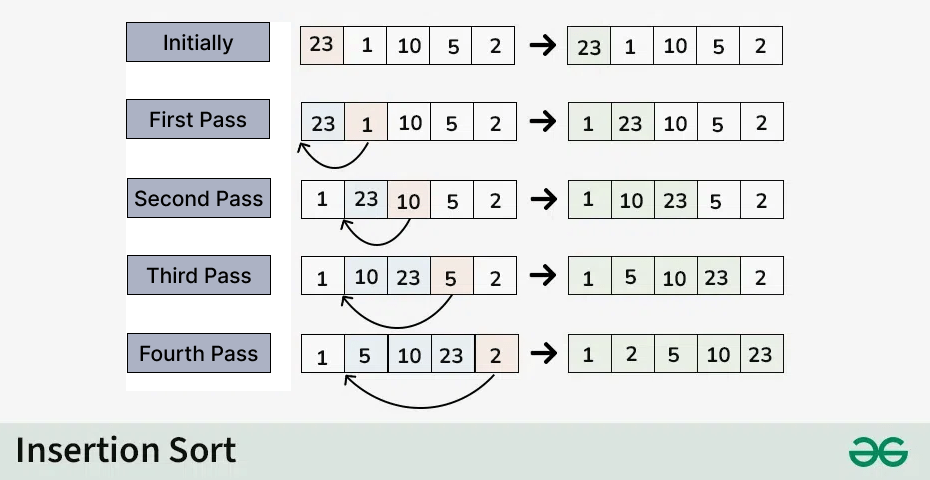
\includegraphics[width=\textwidth]{images/Insertion-sorting.png}
Image Source: https://www.geeksforgeeks.org/insertion-sort-algorithm/

The first element is already considered sorted. For the second element, you must compare against 1 element to decide where to put it; the third requires 2 comparisons; this pattern continues until the last comparison, which would be against $n-1$ elements. The formula $1+2+...+n-1$, when removing constants, also reduces to a Big-O of $O(n^2)$.

\subsubsection{Quick Sort}

Quick Sort is a little more complex, but it is faster than the previous algorithms, hence the name. Quick sort works by splitting our list around a randomly chosen ``pivot" into two smaller lists for us to sort, where one list is smaller than the pivot and the other list is larger than the pivot. We then split those smaller lists around their own pivots again, resulting in four lists. This continues until we run out of elements in our lists.

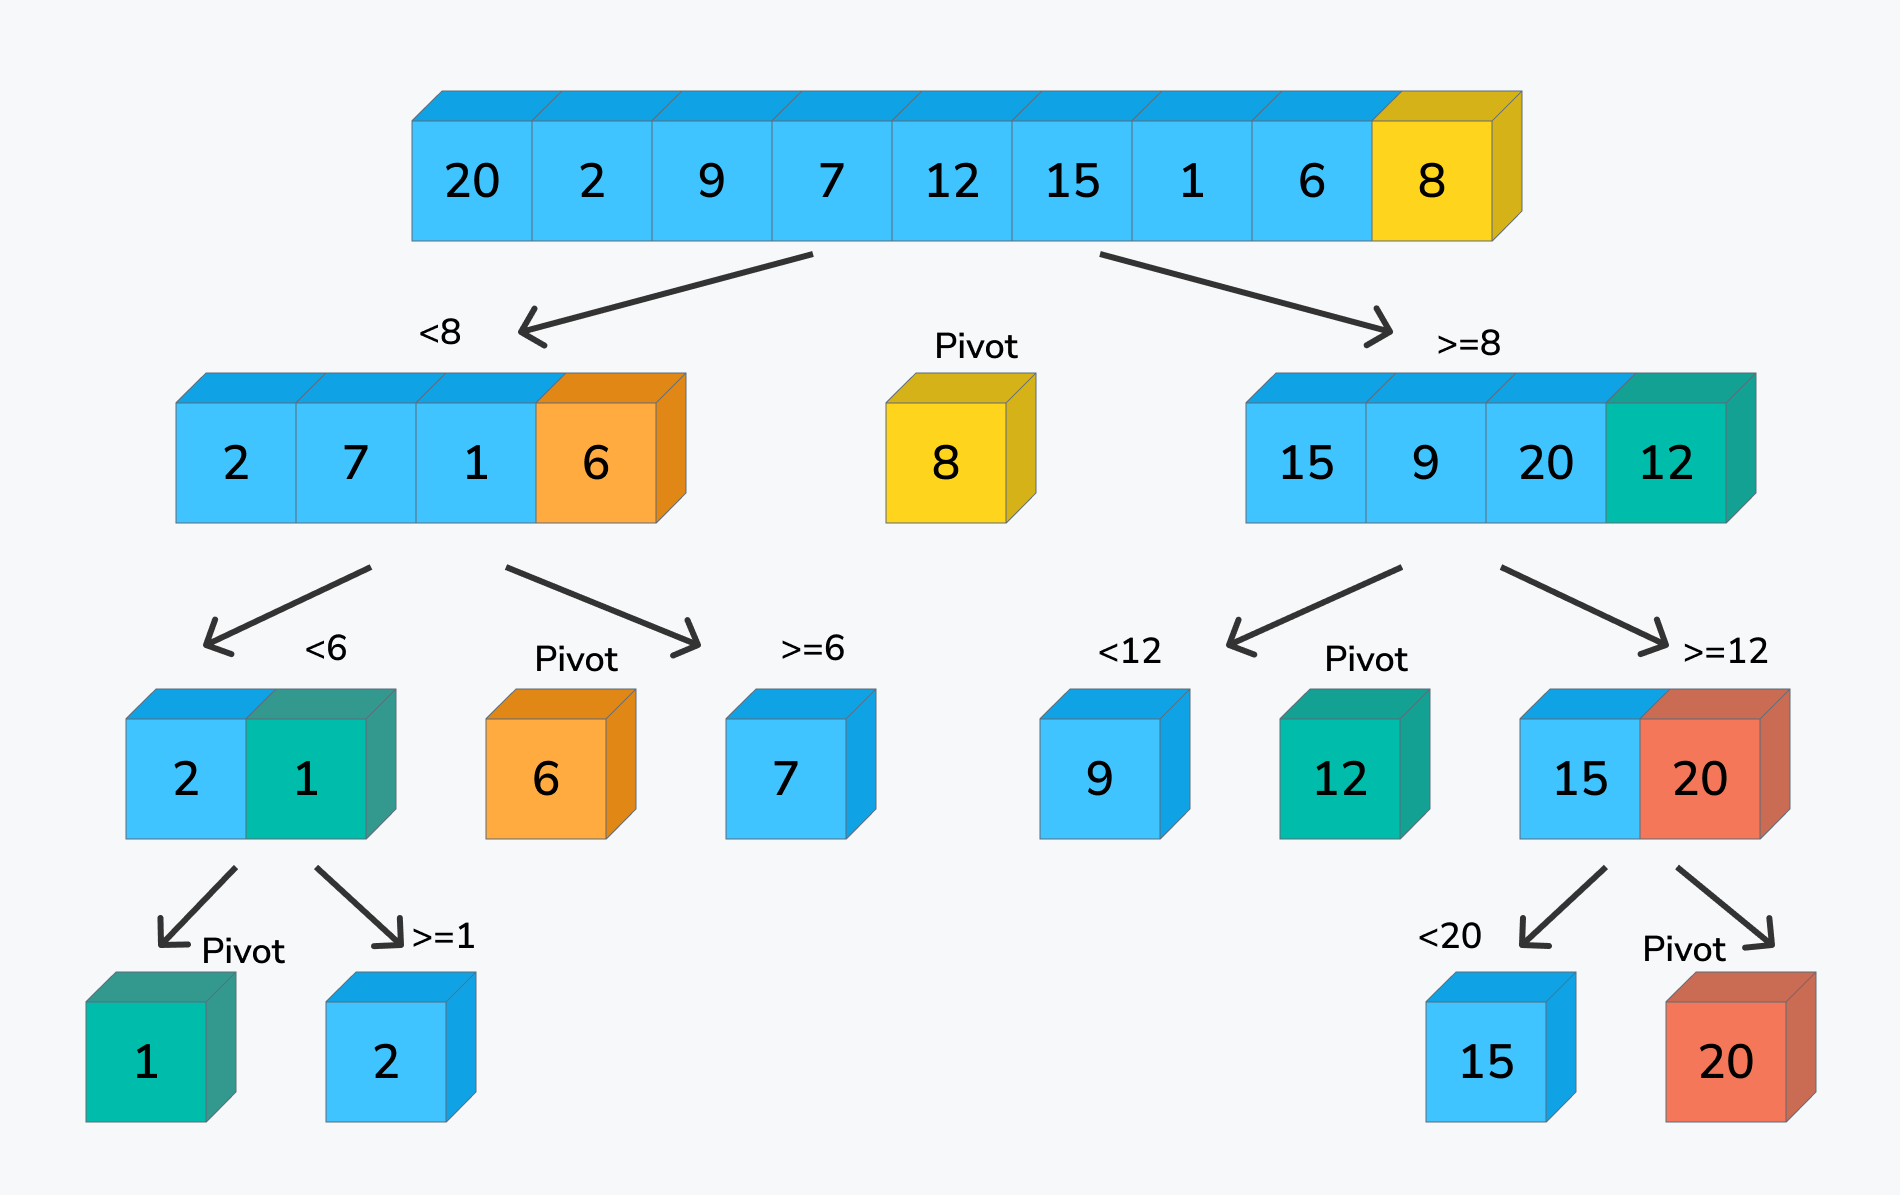
\includegraphics[width=\textwidth]{images/quick-sort.png}

As you can see, this sorting creates a tree-like structure. Each layer contains $n$ elements and requires $n$ operations comparing those elements against their respective pivots. However, the trick that makes this faster than the previous algorithms lies in the number of repetitions for this search: instead of requiring $n$ separate comparisons for each element, as you have seen in the previous three sorting algorithms, you only need as many repetitions as there are layers in this tree. Since each iteration of the tree is splitting the number of elements in half, there are $log(n)$ layers, resulting in a total time complexity of $O(n*log(n))$. 

\subsection{Recursion}
A recursive function is one which calls itself. Recursion can be used to accomplish a repetitive task, like loops. Indeed, it turns out that anything you can do with a loop, you could also do with recursion, and vice versa. However, some algorithms are easier to express with loops, and others are easier to express with recursion. You'll want both in your toolkit to write elegant, simplistic, short code.

Every recursive function includes two parts:

\begin{itemize}
    \item \textbf{base case:} A simple non-recursive occurrence that can be solved directly. Sometimes, there are multiple base cases.
    \item \textbf{recursive case:} A more complex occurrence that can be described using smaller chunks of the problem, closer to the base case.
\end{itemize}
    
To write a recursive function, we often use the following format:

\begin{minted}{c++}
    returnType functionName(arguments)
    {
        if (/*baseCase?*/)
        {
            return /*baseCase result*/;
        }
        else
        {
            // some calculations, including a call to functionName
            // with “smaller” arguments.
            return /*general result*/
        }
    }
\end{minted}

Consider the following simple recursive function, which calculates the sum of the numbers 1, 2, 3, …, n:

\begin{minted}{c++}
int sumNumsRecursive(int num)
{
    // base case: if the number is 0, we will return 0
    if(num == 0)
    {
        return  0;
    }
    else
    {
        // recursive case: where we try to find the result of the previous step
        return num + sumNumsRecursive(num - 1);
    }
}
\end{minted}

The following examples show the final returned value and intermediate recursive function calls.

For example, if \mintinline{c++}{num = 3}.
recursive call 1: \mintinline{c++}{sumNumsRecursive(3)} will return \mintinline{c++}{3 + sumNumsRecursive(2)} (we are running the else statement since num is 3).
recursive call 2: When \mintinline{c++}{sumNumsRecursive(2)} is called, it will return \mintinline{c++}{2 + sumNumsRecursive(1)}.
recursive call 3: Similarly, \mintinline{c++}{sumNumsRecursive(1)} will \mintinline{c++}{return 1 + sumNumsRecursive(0)}.
recursive call 4: Finally, \mintinline{c++}{sumNumsRecursive(0)} will return 0, by definition of the base case.

Next if we go back the chain and replace \mintinline{c++}{sumNumsRecursive(0)} with 0, we will have \mintinline{c++}{sumNumsRecursive(1) = 1 + 0}. Therefore, \mintinline{c++}{sumNumsRecursive(1) = 1}.
Similarly, \mintinline{c++}{sumNumsRecursive(2) = 2 + sumNumsRecursive(1)}, where \mintinline{c++}{sumNumsRecursive(1) = 1}. Therefore, \mintinline{c++}{sumNumsRecursive(2) = 2 + 1}; thus, \mintinline{c++}{sumNumsRecursive(2) = 3}.
Lastly, \mintinline{c++}{sumNumsRecursive(3) = 3 + 3}; the second 3 is the result of \mintinline{c++}{sumNumsRecursive(2)}. Therefore, \mintinline{c++}{sumNumsRecursive(3) = 6}.

Below is the same explanation in a different format.

\begin{verbatim}
sumNumsRecursive(3) = 3 + sumNumsRecursive(2) // running the else statement
                    = 3 + 2 + sumNumsRecursive(1) 
                    // sumNumsRecursive(2) = 2 + sumNumsRecursive(1)
                    = 3 + 2 + 1 + sumNumsRecursive(0) 
                    // sumNumsRecursive(1) = 1 + sumNumsRecursive(0)
                    = 3 + 2 + 1 + 0 
                    // sumNumsRecursive(0) = 0 (base case)
                    = 6
\end{verbatim}


\section{Homework 9}

\textbf{Warning: You are not allowed to use global variables for this assignment.}

This homework is extra credit, you will receive credit for the questions you have completed. 

All function names, return types, and parameters must precisely match those shown. You may not use pass by reference or otherwise modify the function prototypes. You are welcome to create additional functions that may help streamline your code.


\subsection{Carbon Emission Reduction} 
\textit{This question may require the use of recursion, logical and relational operators, if-else statements, declaring and calling a function, and processing user input. Note: you are not allowed to use loops for this question.} \newline

You are tasked with estimating the future reduction in your organization's carbon emissions. Based on historical data, the reduction of carbon emissions for the next year can be predicted from the current year using the following equation:
\begin{equation*}
\text{next\_year\_reduction} = \text{current\_reduction} + 0.5 \times \text{current\_reduction} + 10
\end{equation*}
Develop a recursive function that takes the current year's carbon emission reduction and the number of years forward for which the reduction needs to be predicted and returns the estimated reduction. 

\renewcommand{\arraystretch}{1.5} 
\begin{longtable}{|p{1.7in}|p{4.3in}|}
\hline
\textbf{Function:}  \texttt{emissionReduction(double, int)}& \mintinline{c++}{double emissionReduction(double current_reduction, int years)}\\ \hline

\textbf{Purpose:} & To estimate future reductions in carbon emissions based on current reduction efforts and projected yearly improvements.\\ \hline

\textbf{Parameters:} & 
\textbf{double} \texttt{current\_reduction} - The current year's reduction in carbon emissions. \newline
\textbf{int} \texttt{year} - number of years forward\\ \hline

\textbf{Return Value:} & 
Returns the estimated reduction in carbon emissions after the specified number of years.\\ \hline

\textbf{Error Handling:} & 
- If \texttt{current\_reduction} and/or \texttt{year} is negative, -1 is returned. \newline
- If \texttt{year} is equal to 0, return original \texttt{current\_reduction} \newline
- It should not print anything.\\ \hline

\textbf{Example:}& 

Note: This is only an example of the function; you need to develop your own main function to fulfill the requirement for this problem.

Sample Code:

\begin{example}
        \begin{minted}[breaklines=true]{c++}

// Assume the proper libraries are included.
// Assume the proper implementation of emissionReduction() is included.

int main()
{
    cout << "Predicted reduction in carbon emissions: " << emissionReduction(100, 3) << endl;
    return 0;
}
        \end{minted}
        \end{example}

        \begin{sample}
Predicted reduction in carbon emissions: 385
        \end{sample}\\\hline
\end{longtable}
 
\textbf{For Question 1, develop and validate your solution in VS Code. Once you are happy with your solution, go to coderunner on Canvas and paste emissionReduction() and any helper function(s) to the answer box!}

\begin{sample}
\textcolor{red}{Inputs:}

Current reduction: 200 \newline
Years: 5

\textcolor{red}{Output:}

Predicted reduction in carbon emissions: 444.204

\textcolor{red}{Explanation:}

emissionReduction(200, 0) = 200 \newline
emissionReduction(200, 1) = 200 + 0.5 * 200 + 10 = 310 \newline
emissionReduction(200, 2) = 310 + 0.5 * 310 + 10 = 475\newline
emissionReduction(200, 3) = 475 + 0.5 * 475 + 10 = 722.5 \newline
emissionReduction(200, 4) = 722.5 + 0.5 *722.5 + 10 = 1093.75 \newline
emissionReduction(200, 5) = 1093.75 + 0.5 * 1093.75+ 10 = 1650.62

\end{sample}


\subsection{Vector Shuffle} 
\textit{This question may require the use of functions, vectors, and loops.}

Your task is to write a C++ function that takes the elements of two vectors and returns a vector of integer values that combines the two input vectors by alternating between values from each of the two vectors. If the vectors are of different sizes, the remaining elements from the longer vector should be appended to the result vector.

\renewcommand{\arraystretch}{1.5} 
\begin{longtable}{|p{1.7in}|p{4.3in}|}
\hline
\textbf{Function:}  \texttt{vectorShuffle(vector<int>, vector<int>)}& \mintinline{c++}{vector<int> vectorShuffle(vector<int> vec1, vector<int> vec2)}\\ \hline

\textbf{Purpose:} & To shuffle the elements of two vectors and return a new vector containing elements from both vectors in an interleaved fashion.\\ \hline

\textbf{Parameters:} & 
\textbf{vector<int>} \texttt{vec1} - The first vector of integers \newline
\textbf{vector<int>} \texttt{vec2} - The second vector of integers\\ \hline

\textbf{Return Value:} & 
- \textbf{vector<int>} Returns a new vector containing elements from both \texttt{vec1} and \texttt{vec2} 
\newline
- The function should not print anything.\\ \hline

\textbf{Error Handling:} & 
- If one vector is shorter than the other (including size 0), alternate as long as you can and append the remaining elements from the longer vector. \newline
- If both vectors are empty (size 0), the return value should be an empty vector. \newline
- The first element of the returned vector should come from the first input argument.\\ \hline

\textbf{Example:}& 

Note: This is only an example of the function; you need to develop your own main function to fulfill the requirement for this problem.

Sample Code:

\begin{example}
        \begin{minted}[breaklines=true]{c++}

// Assume the proper libraries are included.

// Assume the proper implementation of vectorShuffle() is included.

int main()
{
    vector<int> vec1 = {1, 3, 5};
    vector<int> vec2 = {2, 4, 6, 8, 10};
    vector<int> result = vectorShuffle(vec1, vec2);
    if (result.size() == 0)
    {
        cout << "No elements found" << endl;
    }
    else
    {
        cout << "Shuffled vector:" << endl;
        for (int i = 0; i < int(result.size()); i++)
        {
            cout << result.at(i) << " ";
        }
        cout << endl;
    }
    return 0;
}
        \end{minted}
        \end{example}

        \begin{sample}
Shuffled vector: \newline
1 2 3 4 5 6 8 10
        \end{sample}\\\hline
\end{longtable}
 
\textbf{For Question 2, develop and validate your solution in VS Code. Once you are happy with your solution, go to coderunner on Canvas and paste the vectorShuffle() and any helper function(s) into the answer box!!}

\begin{sample}
\textcolor{red}{Inputs:}

vector<int> vec1; \newline
vector<int> vec2 = {2, 4, 6, 8, 10};

\textcolor{red}{Output:}

Shuffled vector: \newline
2 4 6 8 10

\end{sample}


\begin{sample}
\textcolor{red}{Inputs:}

vector<int> vec1; \newline
vector<int> vec2;

\textcolor{red}{Output:}

No elements found

\end{sample}
\begin{sample}
\textcolor{red}{Inputs:}

vector<int> vec1 = {1, 1, 3};\newline
vector<int> vec2 = {2, 4, 6, 8, 10};

\textcolor{red}{Output:}

Shuffled vector: \newline
1 2 1 4 3 6 8 10

\end{sample}


\subsection{The Magical List}  
\textit{This question may require the use of functions, vectors, and loops.}

Alex is a curious programmer who loves solving puzzles. One day, while tinkering with numbers, Alex decides to create a magical list that follows a set of peculiar rules. Here's how the game works:

Alex starts with an empty list. They ask a friend to keep entering positive integers, one at a time. The program will continuously prompt the user with ``Please enter a number:" until -1 is entered and each number influences the list in some way:

\begin{enumerate}
    \item If the list is empty, Alex adds the number to the list immediately.
    \item If the number is divisible by both 3 and 5, Alex does both: remove the first and last numbers from the list (if there is a number). 
    \item If the number is divisible by 5, Alex removes the first number from the list (if there is one).
    \item If the number is divisible by 3, Alex removes the last number from the list (if there is one).
    \item If none of the above applies, Alex simply adds the number to the end of the list.
\end{enumerate}

However, there's a catch! If someone enters a negative number that isn't \verb|-1|, or zero, Alex scolds them with:  
\textbf{``The number should be a positive integer or -1."}

When someone finally enters \verb|-1|, Alex stops the game. Then, Alex proudly displays the final list of numbers, separated by spaces. Note: the printing will happen in main(). 

\renewcommand{\arraystretch}{1.5} 
\begin{longtable}{|p{1.7in}|p{4.3in}|}
\hline
\textbf{Function:}  \texttt{processMagicalList()}& \mintinline{c++}{vector<int> processMagicalList()}\\ \hline

\textbf{Purpose:} & To process a series of user inputs according to the rules and return the final list of integers. \\ \hline

\textbf{Parameters:} & 
None. All inputs are provided by the user interactively during execution. \\ \hline

\textbf{Return Value:} & 
\textbf{vector<int>} Returns a vector containing the final list of numbers after applying the rules.\\ \hline

\textbf{Error Handling:} & 
- The program should prompt the user with ``Please enter a number:" for each input. \newline
- If the user enters a non-positive number (excluding \verb|-1|), display \texttt{"The number should be a positive integer or -1."}. \newline
- The function should not print the vector. Printing should be handled by the main function. \\ \hline

\textbf{Example:}& 

Note: This is only an example of the function; you need to develop your own main function to fulfill the requirement for this problem.

Sample Code:

\begin{example}
        \begin{minted}[breaklines=true]{c++}

// Assume the proper libraries are included.

// Assume the proper implementation of processMagicalList() is included.

int main()
{
    vector<int> result = processMagicalList();
    if (result.size() == 0)
    {
        cout << "The vector is empty." << endl;
    }
    else
    {
        cout << "The elements in the vector are: ";
        for (int i = 0; i < int(result.size()); i++)
        {
            cout << result[i] << " ";
        }
        cout << endl;
    }
    return 0;
}
        \end{minted}
        \end{example}

        \begin{sample}
The elements in the vector are: \newline
8
        \end{sample}\\ \hline
\end{longtable}
 
\textbf{For Question 3, develop and validate your solution in VS Code. Once you are happy with your solution, go to coderunner on Canvas and paste the processMagicalList() function into the answer box!}

\begin{sample}
\textcolor{red}{Inputs:}

3, 5, 15, 8, -1

\textcolor{red}{Output:}

Please enter a number: \newline
Please enter a number: \newline
Please enter a number: \newline
Please enter a number: \newline
Please enter a number: \newline
The elements in the vector are: \newline
8

\textcolor{red}{Explanation:}

1. \textbf{3:} The list is empty, so 3 is added to the list. \newline
   Current list: [3] \newline

2. \textbf{5:} The number is divisible by 5. The first number, 3, is removed from the list. \newline
   Current list: [] (empty) \newline

3. \textbf{15:} The number is divisible by both 3 and 5. Since the list is empty, nothing is removed. 15 is added to the list. \newline
   Current list: [15] \newline

4. \textbf{8:} The list is not empty, so 8 is added to the end of the list. \newline
   Current list: [15, 8] \newline

5. \textbf{-1:} The game ends. The list contains numbers, so the program prints the elements: ``The elements in the vector are: 8''. \newline
   Final list: [8]
\end{sample}

\begin{sample}
\textcolor{red}{Inputs:}

0 -5 6 -1

\textcolor{red}{Output:}
Please enter a number: \newline
The number should be a positive integer or -1. \newline
Please enter a number: \newline
The number should be a positive integer or -1. \newline
Please enter a number: \newline
Please enter a number: \newline
The elements in the vector are: \newline
6

\end{sample}

\begin{sample}
\textcolor{red}{Inputs:}

10, 9, 4, -1

\textcolor{red}{Output:}

Please enter a number: \newline
Please enter a number: \newline
Please enter a number: \newline
Please enter a number: \newline
The elements in the vector are: \newline
4

\textcolor{red}{Explanation:}

1. \textbf{10:} The number is divisible by 5. The first number in the list is removed. Since the list is empty, nothing happens. \newline
   Current list: [] (empty) \newline

2. \textbf{9:} The number is divisible by 3. The last number in the list is removed. Since the list is empty, nothing happens. \newline
   Current list: [] (empty) \newline

3. \textbf{4:} The number is not divisible by 3 or 5, so it is added to the end of the list. \newline
   Current list: [4] \newline

4. \textbf{-1:} The game ends. The program prints: ``The elements in the vector are: 4''. \newline
   Final list: [4]
\end{sample}


\subsection{T Ball Players} 
\textit{This question may require the use of arrays, logical and relational operators, if-else statements, declaring and calling a function.}

Coach Prime is getting ready for the new T-ball season and needed to finalize his roster. The team is open to kids between the ages of 4 and 6, and parents had already sent in names and ages of their children. 

Write a function, printEligiblePlayers, to help Coach Prime filter out the eligible players from the list of names and ages. Your function should identify players between 4 and 6 years old (inclusive) and print their names along with their ages, so Prime Kelly can focus on training her future stars.

\textbf{Function Specification :}

\renewcommand{\arraystretch}{1.5} 
\begin{longtable}{|p{1.7in}|p{4.3in}|}
\hline
\textbf{Function:}  \texttt{printEligiblePlayers(string, double, int)}& \mintinline{c++}{void printEligiblePlayers(string names[], double ages[], int num)}\\ \hline

\textbf{Purpose:} & To identify players between 4 and 6 years old (inclusive) and print their names along with their ages\\ \hline

\textbf{Parameters:} & 
\textbf{string} \texttt{names[]} - an array of strings to hold names of players \newline
\textbf{double} \texttt{ages[]} - an array of floating point numbers (as doubles) to hold ages of players \newline
\textbf{int} \texttt{num} - an integer that gives the number of elements in the players and ages arrays
\\ \hline

\textbf{Return Value:} & 
The function does not return anything\\ \hline

\textbf{Error Handling:} & 
- The size of names and ages will be the same represented by num.\\ \hline

\textbf{Example:}& 

Note: This is only an example of the function; you need to develop your own main function to fulfill the requirement for this problem.

Sample Code:

\begin{example}
        \begin{minted}[breaklines=true]{c++}

// Assume the proper libraries are included.
// Assume the proper implementation of printEligiblePlayers() is included.

int main()
{
    string names[4] = {"Joe", "Jack", "Amy", "Bob"};
    double ages[4] = {4.0, 5.6, 6.0, 4.2};
    printEligiblePlayers(names, ages, 4);
}
        \end{minted}
        \end{example}

        \begin{sample}
Joe 4 \newline
Jack 5.6 \newline
Amy 6 \newline
Bob 4.2

        \end{sample}\\\hline
\end{longtable}
 
\textbf{For Question 4, develop and validate your solution in VS Code. Once you are happy with your solution, go to coderunner on Canvas and paste printEligiblePlayers() and any helper function(s) to the answer box!}

\begin{sample}
\textcolor{red}{Inputs:}

string names[4] = {"Joe", "Jack", "Amy", "Bob"}; \newline
double ages[4] = {3.4, 5.6, 6.4, 4.2}; \newline
printEligiblePlayers(names, ages, 4); \newline


\textcolor{red}{Output:}

Jack 5.6 \newline
Bob 4.2

\end{sample}


\subsection{Music App} 

For this question, you'll develop a basic Music App System by creating a Library class to manage a collection of songs. For this question, you will create a Song class. 

The \textbf{Song} class comprises the following attributes:

\vspace{10pt}

\textbf{Data members (private)}

\renewcommand{\arraystretch}{1.5}
\begin{longtable}{|p{1.5in}|p{1.5in}|p{2.9in}|}
\hline
\textbf{Member Type} & \textbf{Member Name} & \textbf{Description} \\ \hline

\mintinline{c++}{string} & \mintinline{c++}{_title}& The name of the song\\ \hline

\mintinline{c++}{string}& \mintinline{c++}{_artist}& The name of the song who sang the song\\ \hline

\mintinline{c++}{int} & \mintinline{c++}{_downloads}& A count of the number of times the song was download\\\hline

\end{longtable}

\textbf{Member Functions (public)}

\renewcommand{\arraystretch}{1.5} 
\begin{longtable}{|p{2.0in}|p{4.0in}|}
\hline
\textbf{Function} & \textbf{Description} \\ \hline

\texttt{Default constructor} & Creates a new instance of \mintinline{c++}{Song} by setting \mintinline{c++}{_title} to an empty string,  \mintinline{c++}{_artist} to an empty string and  \mintinline{c++}{_downloads} to 0.\\ \hline

\mintinline{c++}{Song(string)}& Creates a new instance of \mintinline{c++}{Song} by setting \mintinline{c++}{_title} as the string parameter,  \mintinline{c++}{_artist} to an empty string and  \mintinline{c++}{_downloads} to 0.\\ \hline

\mintinline{c++}{Song(string, string, int)}& Creates a new instance of \mintinline{c++}{Song} by setting \mintinline{c++}{_title} as the first string parameter,  \mintinline{c++}{_artist} as the second string parameter and  \mintinline{c++}{_downloads} to the integer parament. See Function Specification table below for more details.\\ \hline

\mintinline{c++}{string getTitle()}& Returns the \mintinline{c++}{_title} of the \mintinline{c++}{Song}.\\ \hline

\mintinline{c++}{string getArtist();}& Returns the \mintinline{c++}{_artist} of the \mintinline{c++}{Song}.\\ \hline 
 \mintinline{c++}{int getDownloads();}&Returns the 
 number of \mintinline{c++}{_downloads} of the \mintinline{c++}{Song}.\\\hline \hline

\mintinline{c++}{void setTitle(string)}& Sets the \mintinline{c++}{_title} to the value of the provided string parameter.\\ \hline

\mintinline{c++}{void setArtist(string)}& Sets the \mintinline{c++}{_artist} to the value of the provided string parameter.\\ \hline

\mintinline{c++}{void setDownloads(int)}& Sets the \mintinline{c++}{_downloads} to the value of the provided int parameter.\\ \hline

\mintinline{c++}{double grossRevenue(double)} & 
Calculates the revenue generated by the \mintinline{c++}{Song} by taking in a price per download and returning the total revenue. 
Formula: \(\text{revenue} = \text{price} \times \_downloads\). See the Function Specification table below for more details. \\ \hline


\end{longtable}


\textbf{Function Specifications:}

\renewcommand{\arraystretch}{1.5}
\begin{longtable}{|p{1.7in}|p{4.3in}|}
\hline
\textbf{Function:} \mintinline{c++}{Song(string, string, int)}& \mintinline{c++}{Song(string title, string artist, int downloads)}\\ \hline

\textbf{Purpose:} & This parameterized constructor creates a new instance of the \mintinline{c++}{Song} class. \newline
- Sets \mintinline{c++}{_title} to \mintinline{c++}{title}. \newline
- Sets \mintinline{c++}{_artist} to \mintinline{c++}{artist} \newline
Sets \mintinline{c++}{_downloads} to \mintinline{c++}{downloads}\\ \hline

\textbf{Parameters:} & 
\mintinline{c++}{string} \mintinline{c++}{title} - The title of the Song. \newline
\mintinline{c++}{string} \mintinline{c++}{artist} - The artist who sang the Song. \newline
\mintinline{c++}{int} \mintinline{c++}{downloads} - Number of times the songs has been downloaded. \\ \hline

\textbf{Return Value:} & N/A \\ \hline

\textbf{Error Handling:} & 
- If the \mintinline{c++}{downloads} count is non-positive, set \_download to 0. \\ \hline

\textbf{Example:} & 


\begin{example}


\begin{minted}[breaklines=true]{c++}

// Assume the proper libraries are included
// Assume the proper implementation of the class is included

int main() {
    string title = "Aint Got It Like That";
    string artist = "Earl St. Clair";
    int downloads = 5;
    Song new_song = Song(title, artist, downloads);
}
\end{minted}
\end{example}

\textbf{Expected Contents of \mintinline{c++}{new_song} Object:}

\vspace{5pt}
\mintinline{c++}{_title} = ``Aint Got It Like That" \newline
\mintinline{c++}{_artist} = ``Earl St. Clair"
\newline
\mintinline{c++}{_downloads} = 5
\vspace{5pt}\\ \hline
\end{longtable}


\renewcommand{\arraystretch}{1.5}
\begin{longtable}{|p{1.7in}|p{4.3in}|}
\hline
\textbf{Function:} \mintinline{c++}{double grossRevenue(double)}& \mintinline{c++}{double grossRevenue(double price)}\\ \hline

\textbf{Purpose:} & Calculates the revenue generated by the \mintinline{c++}{Song} using the formula: revenue = price x \_downloads. \\ \hline

\textbf{Parameters:} & 
\mintinline{c++}{int} \mintinline{c++}{price} - The price per download of a song.\\ \hline

\textbf{Return Value:} & \mintinline{c++}{double} : Returns a double representing the revenue generated from the \mintinline{c++}{Song} downloads.\\ \hline

\textbf{Error Handling:} & 
- If the \mintinline{c++}{price} amount is non-positive, do not add or modify any contents, and return -1. \newline\\ \hline

\textbf{Example:} & 

\begin{example}

\begin{minted}[breaklines=true]{c++}

// Assume the proper libraries are included
// Assume the proper implementation of the Library class is included

int main() {
    string _title = "Get Schwifty";
    string _artist = "Rick Sanchez";
    int _downloads = 1000;
    double price = 1.1;
    Song new_song = Song(_title, _artist, _downloads);

    cout << fixed<< setprecision(2) << new_song.grossRevenue(price) << endl;
}
\end{minted}
\end{example}

\textbf{Expected Output:} 

\vspace{5pt}
The expected output after the function call:

1100.00\\ \hline

\end{longtable}

\textbf{For Question 4, develop and validate your solution in VS Code. Once you are happy with your solution, go to coderunner and paste the Song Class header (.h file) and all the implementations (.cpp file). Do not include your driver file (main())}

\subsection{College Admission} 
\textit{This question may require the use of file streams, logical and relational operators, if-else statements, declaring and calling a function, and processing user input.}

You are part of a college admission board and have been requested to write a program to recommend prospective students for admission based on specific criteria using data from a text file. Each line in the file contains student data in the format:

\verb|Student Name, SAT, GPA, Interest, High School Quality, Sem1, Sem2, Sem3, Sem4|.

\begin{enumerate}
    \item \textbf{Overall Score Calculation}

Use the following formula to calculate each student’s score:
\[
\text{Score} = (0.4 \times \text{GPA}) + (0.3 \times \frac{\text{SAT}}{1600}) + (0.2 \times \text{High School Quality}) + (0.1 \times \text{Interest})
\]
Students with a score of \textbf{2.5 or higher} are selected under the "score" criteria.

    \item \textbf{Outlier Detection}

Flag students as "outliers" if the interest is 0 and they have a score of 1.5 or higher.

    \item \textbf{Grade Improvement Detection}

Students are flagged for "grade improvement" if their semester grades show a consistent increase (i.e., \(Sem1 < Sem2 < Sem3 < Sem4\)) and they have a score of \textbf{1.5 or higher}.

    \item \textbf{Output}

For each student, print their name, score (to 6 decimal places), and the criteria (``score", ``outlier", or ``grade improvement") if applicable. If no criteria are met, print just the name and score.
\end{enumerate}

\textbf{Required Functions :}

\begin{itemize}
    \item Use a predefined \verb|split()| function available on Canvas to parse the file.
    \item Implement the \verb|processAdmission()| function to handle calculations and criteria checking.
    \item Hint: you may use the to\_string function to convert numbers (int, double) into strings. For example, \mintinline{c++}{string example = to_string(1.0);}. 
\end{itemize}
 
\textbf{Function Specification :}

\renewcommand{\arraystretch}{1.5} 
\begin{longtable}{|p{1.7in}|p{4.3in}|}
\hline
\textbf{Function:}  \texttt{string processAdmission(string)}& \mintinline{c++}{string processAdmission(string line)}\\ \hline

\textbf{Purpose:} & To analyze a student's data, calculate their admission score, and determine whether they meet the criteria for admission based on score, outlier, or grade improvement.\\ \hline

\textbf{Parameters:} & 
\textbf{string} \texttt{line} - A single line of comma-separated student data containing the student’s name, SAT, GPA, interest, high school quality, and semester grades. \newline
Note: we have skipped the header in main(); therefore, you may assume that all \mintinline{c++}{line} that are passed can be parsed.\\ \hline

\textbf{Return Value:} & 
Returns a string formatted as: \texttt{Name,Score,[criteria]}\\ \hline

\textbf{Error Handling:} & 
- Flag students as "outliers" if Interest = 0 and the score is 1.5 or higher. \newline
- Flag students for "grade improvement" if the grade of each semester is higher than the previous semester and the student has a score of 1.5 or higher. \newline
- Assumes valid input format for the line. The function does not handle cases where the line is improperly formatted or contains invalid data types. \newline
- The function should not print anything.\\ \hline

\textbf{Example:}& 

Note: This is only an example of the function; you need to develop your own main function to fulfill the requirement for this problem.

Sample Code:

\begin{example}
        \begin{minted}[breaklines=true]{c++}

// Assume the proper libraries are included.
// Assume the proper implementation of processAdmission() and split() is included.

int main(){
    string fileName;
    string line;
    
    cout<<"Enter the file name:"<<endl;
    cin>>fileName;
    
    ifstream file(fileName);
    if(file.is_open()){
        cout<<endl<<"Results:"<<endl;
        getline(file, line); // Skip header
        while (getline(file, line)){
            cout << processAdmission(line) << endl;
        }
    } else {
        cout<<"Could not open file."<<endl;
    }
    
    return 0;
}
        \end{minted}
        \end{example}

\begin{sample}
\textcolor{red}{Input:}
text8.txt

\textcolor{red}{File Content:}
\begin{verbatim}
Student,SAT,GPA,Interest,High School Quality,Sem1,Sem2,Sem3,Sem4
Anne Mutant,1550,3.89,0,9,97,87,97,87
Ayla Ranefer,1370,4,3,7,85,86,91,95
\end{verbatim}
\textcolor{red}{Output:}
\begin{verbatim}
Results:
Anne Mutant,3.646625,score
Ayla Ranefer,3.556875,score
\end{verbatim}
        \end{sample}\\\hline
\end{longtable}
 
\textbf{For Question 6, develop and validate your solution in VS Code. Once you are happy with your solution, go to coderunner on Canvas and paste processAdmission(), split() and any helper function(s) to the answer box!}

\begin{sample}
\textcolor{red}{Input:}
file-does-not-exist.txt

\textcolor{red}{File Content:}
//file does not exist
\begin{verbatim}
\end{verbatim}
\textcolor{red}{Output:}
\begin{verbatim}
Could not open file.
\end{verbatim}
        \end{sample}

\begin{sample}
\textcolor{red}{Input:}
text.txt

\textcolor{red}{File Content:}
\begin{verbatim}
Student,SAT,GPA,Interest,High School Quality,Sem1,Sem2,Sem3,Sem4
Abbess Horror,1300,3.61,10,7,95,86,91,94
Anastasia Kravinoff,1500,3.74,0,0,92,86,81,90
Adelicia von Krupp,900,4,5,2,88,92,83,72
Anna Frankenstein,1050,2.42,5,4,90,91,93,98
\end{verbatim}
\textcolor{red}{Output:}
\begin{verbatim}
Results:
Abbess Horror,4.087750,score
Anastasia Kravinoff,1.777250,outlier
Adelicia von Krupp,2.668750,score
Anna Frankenstein,2.464875,grade improvement
\end{verbatim}
        \end{sample}


